\documentclass[12pt]{beamer}
\usetheme{copenhagen}
\usepackage{ifxetex,ifluatex}
\usepackage[T1]{fontenc}
\usepackage{lmodern}
\usepackage[utf8]{inputenc}
\usepackage[spanish,catalan,english]{babel}
\usepackage{hyperref}
\usepackage{color}
\usepackage{array}
\usepackage{amsmath,amssymb,amsfonts,amsthm,mathrsfs,amsbsy}
\usepackage{graphicx}
\usepackage{enumerate}
\usepackage{verbatim}
\usepackage{dsfont}
\usepackage[all]{xy}
\usepackage{hyperref}
\usepackage{layout}
\usepackage{array}
\usepackage{float}
\usepackage{xypic}
\usepackage{tikz,ifthen}
\usepackage{multicol}
\usepackage{multirow}
\usepackage{ragged2e}
\usepackage[3D]{movie15}

\title{01. Instalación Entorno de Desarrollo de Android}
\author{Xavi Lara - Profesor I.Sabadell xlara@ies-sabadell.cat}
\institute{
\includegraphics[scale=0.5]{LogoInstitut.png}}
\date{}

\begin{document}
	\begin{frame}
		\maketitle
	\end{frame}
	\section{1. Instalació d'Android Studio}
	\subsection{1.1. Descarrega de l'Instalador d'Android Studio}
	\subsubsection{1.1.1. Descarrega de l'Instalador d'Android Studio}
	\begin{frame}
		\begin{block}{1.1.1. Descarrega de l'Instalador d'Android Studio}
			Anem a la direcció  \textcolor{blue}{\href{https://developer.android.com/studio}{developer.android.com/studio}} i descarreguem la última versió d'Android Studio.
		\end{block}
		\centering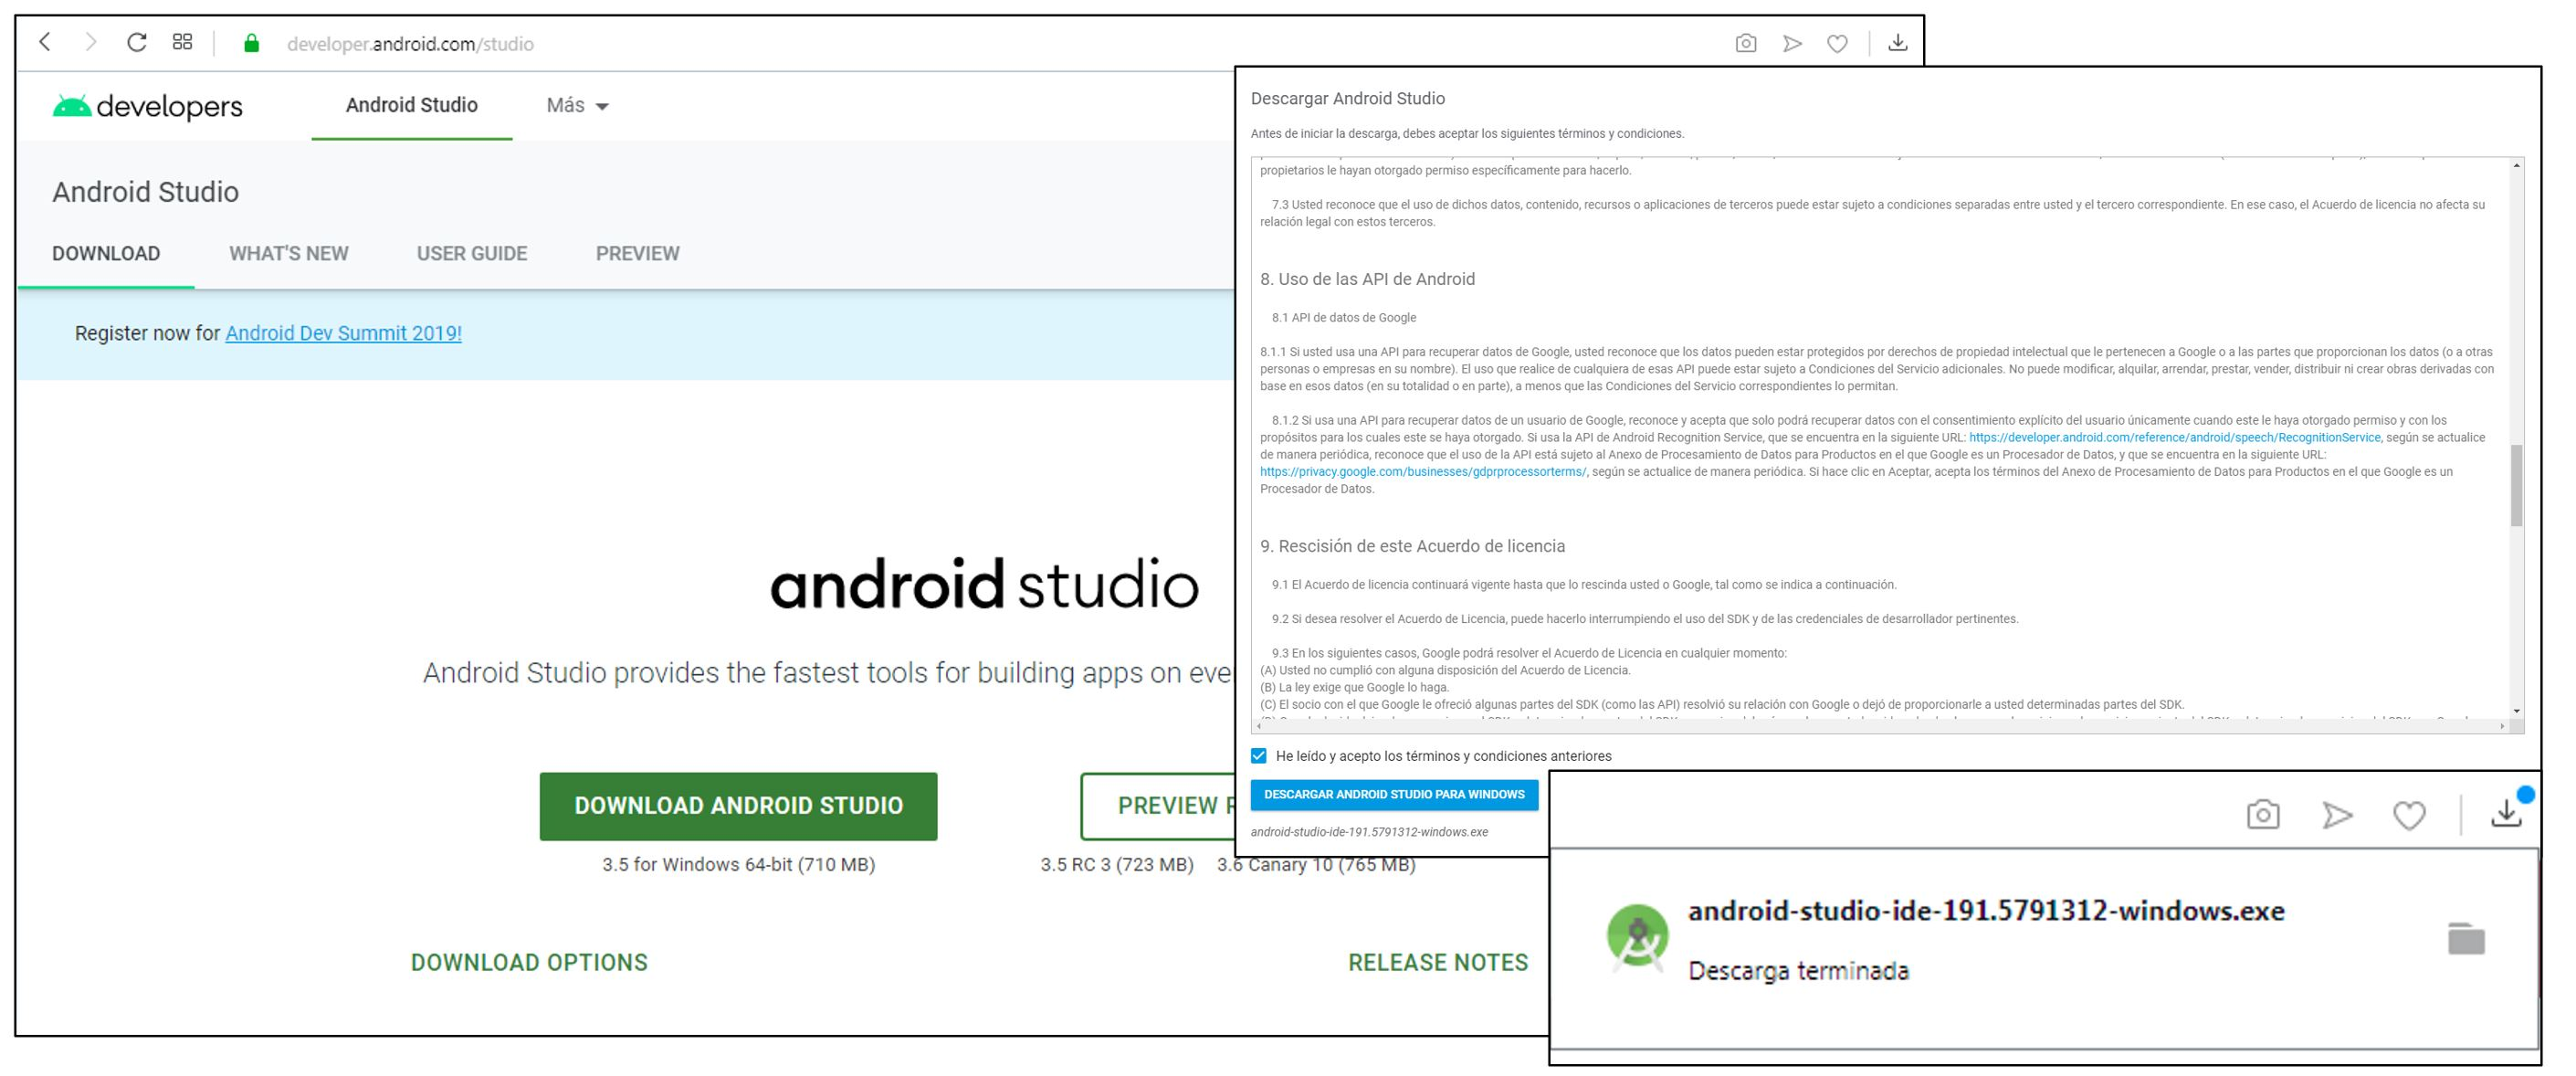
\includegraphics[scale=0.15]{DescargaWeb.JPG}
	\end{frame}
	\subsubsection{1.1.2. Execució de l'Instalador d'Android Studio}
	\begin{frame}	
		\begin{block}{1.1.2. Execució d l'Instalador d'Android Studio}
			Iniciem la instalació d'Android Studio.
		\end{block}
		\centering
		\begin{tabular}{cc}
			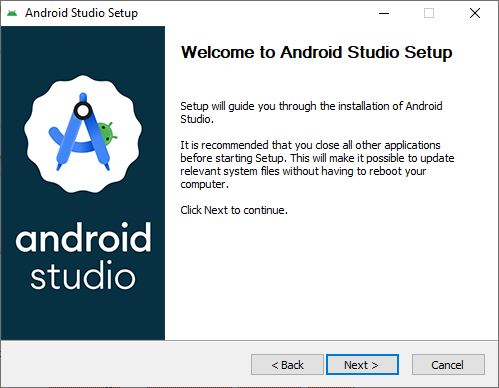
\includegraphics[scale=0.35]{Instalacio01.JPG}&
			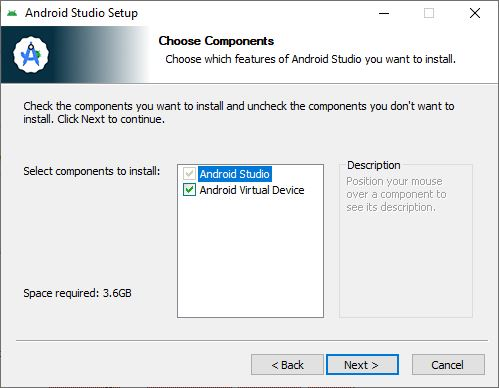
\includegraphics[scale=0.35]{Instalacio02.JPG}\\
			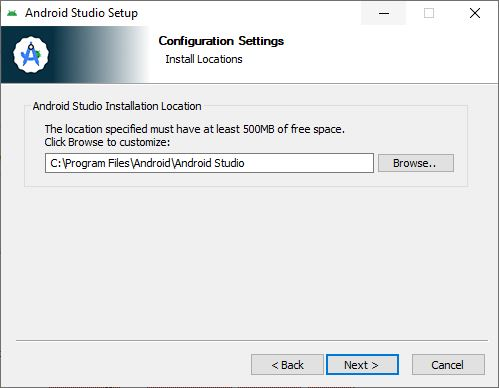
\includegraphics[scale=0.35]{Instalacio03.JPG}&
			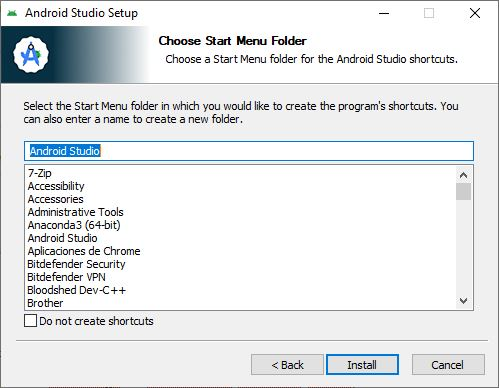
\includegraphics[scale=0.35]{Instalacio04.JPG}\\
		\end{tabular}
	\end{frame}
	\subsubsection{1.1.3. Finalització de l'Instalació d'Android Studio}
	\begin{frame}
		\begin{block}{1.1.3. Finalització de l'Instalació d'Android Studio}
			Finalitzem l'instalació d'Android Studio e inicialitzem.
		\end{block}
		\centering
		\begin{tabular}{cc}
		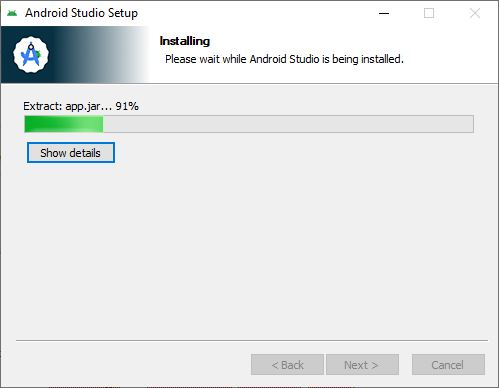
\includegraphics[scale=0.35]{Instalacio05.JPG}&
		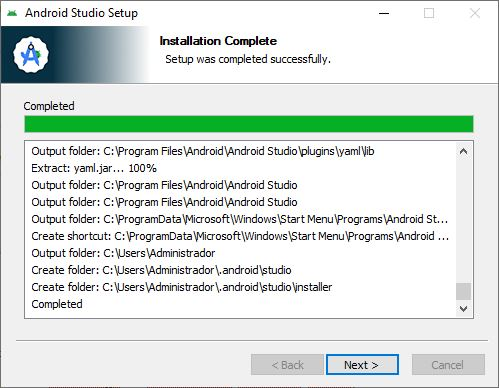
\includegraphics[scale=0.35]{Instalacio06.JPG}\\
		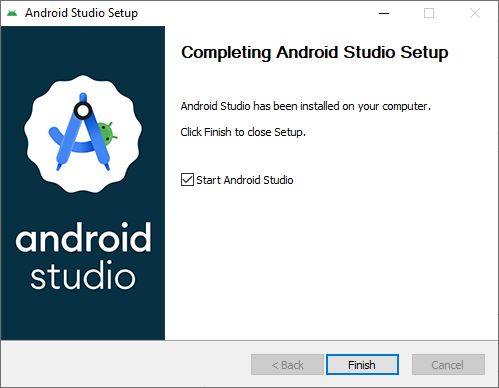
\includegraphics[scale=0.35]{Instalacio07.JPG}&
		
\includegraphics[scale=0.30]{Instalacio08.JPG}\\
		\end{tabular}
	\end{frame}
	\section{2. Creació de Nou Projecte}
	\subsection{2.1. Creació de Nou Projecte}
	\subsubsection{2.1.1. Menú d'Inici de Android Studio.}
	\begin{frame}
		\begin{block}{2.1.1. El Menú d'Inici de Android Studio.}
			Al iniciar Android Studio s'ens obra el menú de projectes.
		\end{block}
		\centering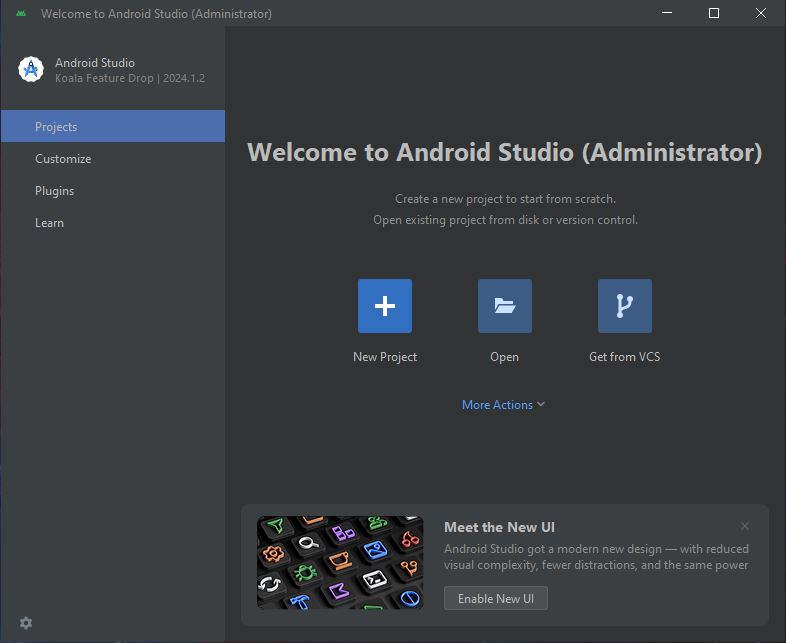
\includegraphics[scale=0.4]{NewProject01.JPG}\\
	\end{frame}
	\subsubsection{2.1.2. Comencem Nou Projecte}
	\begin{frame}
		\begin{block}{2.1.2. Comencem Nou Projecte}
			Seleccionem un nou projecte amb la plantilla Empty Activity.
		\end{block}
		\centering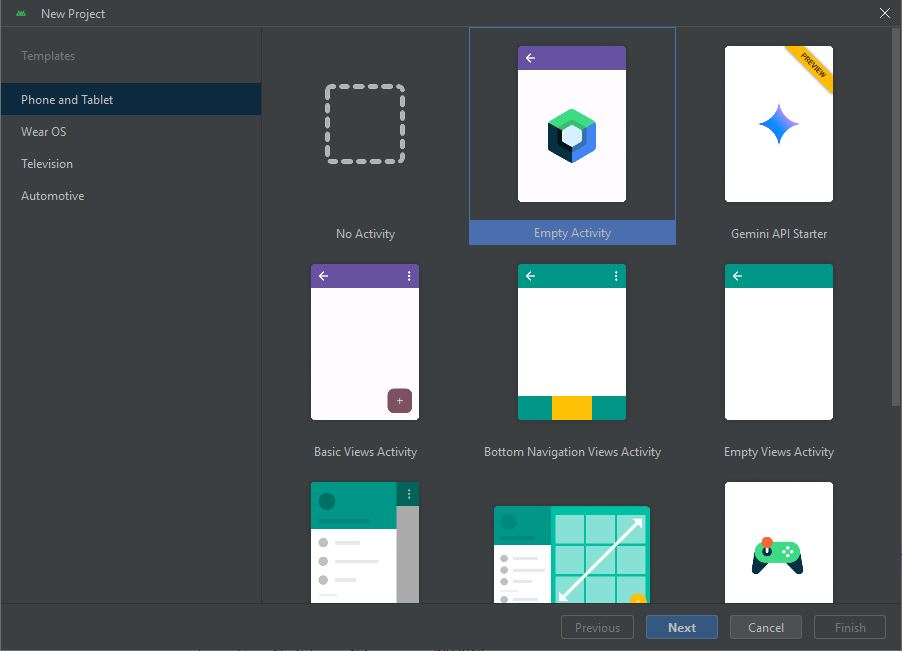
\includegraphics[scale=0.4]{NewProject02.JPG}\\
	\end{frame}
	\subsubsection{2.1.3. Configuració del Nou Projecte}
	\begin{frame}
		\begin{block}{2.1.3. Configuració del Nou Projecte}
			Aquest projecte será en llenguatge Kotlin.
		\end{block}
		\centering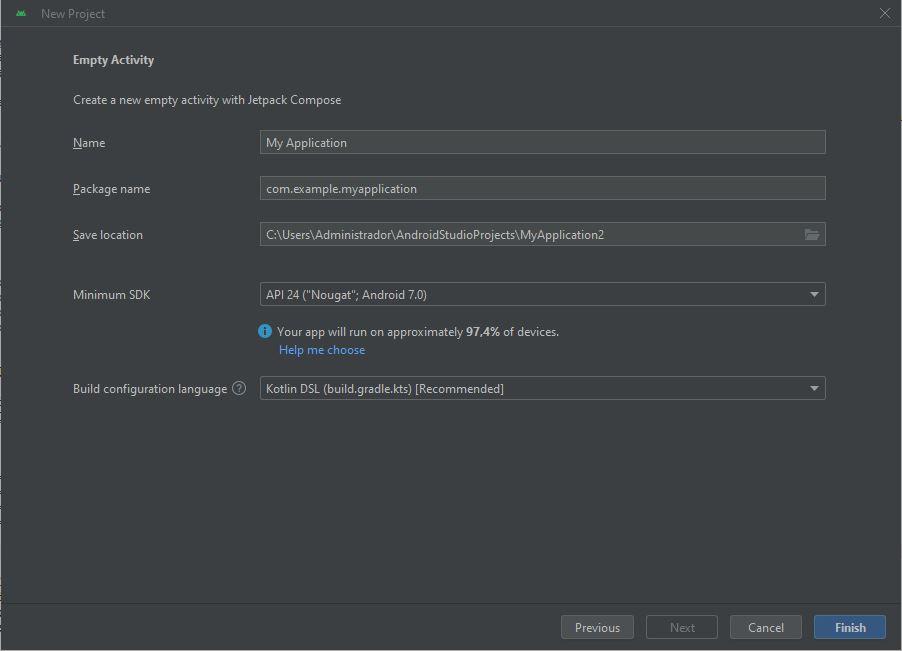
\includegraphics[scale=0.4]{NewProject03.JPG}
	\end{frame}
	\section{3. Configuració d'Android Studio}
	\section{4. Execució d'Aplicació}
	\section{5. Emulador de Android Studio}
	\section{6. Execució al Dispositiu Mòbil}
\end{document}
